\documentclass[12pt]{article}
\usepackage[utf8]{inputenc}

\usepackage{geometry}
\usepackage{setspace}
\usepackage{amsmath}

\geometry{margin=.95in}
\onehalfspacing

\title{\textsc{}\\A basic insurance model for decentralized insurance\\\textit{V0.3}}
\author{Jake Brukhman\\ \texttt{jake@coinfund.io}}
\date

\usepackage{natbib}
\usepackage{graphicx}

\usepackage{titling}
\pretitle{\begin{flushright}\LARGE}
\posttitle{\par\end{flushright}\vskip 0.5em}
\preauthor{\begin{flushright}\small \lineskip 0.5em}
\postauthor{\par\end{flushright}}
\predate{\begin{flushright}\large}
\postdate{\par\end{flushright}}

\usepackage{float}

\usepackage{graphicx}
\graphicspath{ {images/} }

\begin{document}

\maketitle

\section{Introduction}

In this work, we attempt to describe the mathematics of a basic insurance scheme with an eye toward implementation as prototype of a decentralized insurance product based on Ethereum\footnote{http://ethereum.org} or another similar smart contract platform. The prospect of implementing insurance as a smart contract is compelling in at least two ways. First and foremost, insurance companies are typically traditional centralized organizations which have to figure in hefty operational costs into their offerings, premiums, and measures of performance. The concept of \textit{combined ratio} is a measure of profitability insurance companies use to indicate how well they are performing and operating;\footnote{http://www.investopedia.com/terms/c/combinedratio.asp}In the context of smart contract insurance, we use the benefit of automation to bring the expense outflow of this measure effectively to 0. The second benefit of considering smart contracts as an insurance platform deals with the flexibility of digital assets: using smart contract as a toolkit for decentralized economics, we are free to explore possibilities of reinsurance markets with completely customized token economics and a global investor market.

In Section 2, we develop the mathematics for a basic insurance model based on a sum of independent Bernoulli random variables with a fixed payout $P^*$ for each policy. We will present the methodology for calculating the insurance premium, $P$, and for ascertaining the collateralization necessary to increase the probability of solvency of the insurance pool to an arbitrary confidence level $\pi$. Based on this model, we will describe the revenue and revenue margins of the insurance scheme and calculate the expected risk and return of the scheme. While simple, this model will develop for us a good intuition about the interactions of premiums, payouts, and risk in the smart contract's insurance pool.

In Section 3, we extend our model to a more realistic scenario where insurance payouts $P_i^*$ can vary across policies, and the probability $p_i$ of each event can be parameterized separately. We also present a methodology for determining the premiums $P_i$ corresponding to each $P_i^*$, and provide a strategy for Monte Carlo simulation which attains the necessary model outputs.

Since the insurance pool can be viewed as a form of portfolio with credit risk, and therefore the collateral, $C$, present in the portfolio is typically much lower than the actual total liability, $L$, of the portfolio. As such, the portfolio is susceptible to long-tail events which exhaust the collateral and cause the insurance pool to become insolvent; moreover, these long-tail events often break down models due to correlations which manifest under these adverse conditions. The typical strategy for dealing with long-tail events in an insurance context is by selling long-tail risk to reinsurers, who collect this type of risky exposure in diversified portfolios. However, given our smart contract context, we explore an alternative token-based form of reinsurance that can be offered as a digital asset on global cryptomarkets in Section 4.

\section{A binomial distribution insurance model}

An insurance pool is a capital pool that is intended to provide insurance against some \textit{insurable event}. We do not specify the nature of the event, but we assume that all such events are independent and occur with probability $p$. In an insurance pool, $n$ policies are issued for a premium, denoted $P$.  Each policy holder expects a payout of $P^*$ if the event occurs. Both the independence of insurable events and the constant payout $P^*$ are simplifying assumptions to be expanded upon later.

Immediately, we can define the \textit{return multiple} of a particular insurance scheme as
\begin{equation}
  \label{return}
  r := \frac{P^*}{P}.
\end{equation}
For instance, if $r = 10$ for some insurance scheme, then this scheme will return a payout $10$ times greater than the premium paid. With premiums equal, a rational insurance purchaser should prefer an insurance scheme with greater $r$ to a scheme with a smaller $r$. It is also useful to note that $r$ is a function of $n$, $r=r(n)$, since usually one of $\{P, P^*\}$ is given a parameter, and the other variable is calculated as an $n$-dependent output of the model.

\subsection{Total liability of the insurance pool}

Let us define
$$L(n) := nP^*\ ;\ \ \ C(n) := nP$$
In general, $L(n)$ denotes the total liability of a Bernoulli insurance pool; namely, it is the amount of capital that the pool would need to pay out if \textit{all} policy payouts were claimed. Instead of collecting enough collateral to cover the total liability of the pool, this scheme uses the knowledge of the probabilities of the insurable events to capitalize against a reasonably improbable minority of claims, as described below. We are also denoting by $C(n)$ the capital pool, or collateral, of the pool. Note that in typical insurance schemes, collateralization is lower than the liability: $C(n)/L(n) < 1$.

\subsection{Binomial distribution insurance scheme}

We can model each policy as independent identically-distributed Bernoulli random variables $X_i$ ($i = 1,\ldots, n$). That is, each $X_i$ takes the value $1$ with probability $p$ (if the event occurs), and the value $0$ with probability $1-p$ if the policy expires without the event taking place. We can abbreviate this condition $P(X_i = 1) = 1 - P(X_i = 0) = p$.

Let us define the sum of these random variables as $X = \sum_{i=1}^n X_i$. Clearly, the random variable $X$ measures the number of claims that the pool will need to pay in the future. It is well known by the additivity of the expectation and variance of independent random variables that
\begin{equation}
  \label{mu}
  \mu = E(X) = np\ ;\ \ \ \sigma = \sqrt{Var(X)} = \sqrt{np(1-p)}
\end{equation}
We now turn to the problem of calculating the relationship between the premium and the payout. Let us suppose that the payout $P^*$ is fixed, and that $P^*\geq P>0$. As we see from (\ref{mu}) above, in the average case, the number of claims is $\mu = np$. If we capitalize the pool with $\mu P^*$ worth of capital, and because that capital is collected from premiums, we have $C(n) = nP \geq \mu P^* = npP^*$, and the following relationship.
\begin{equation}
\label{avgpremium}
P \geq pP^*
\end{equation}
This formula implies that if we collect enough collateral to back the average number of claims, the premium correlates positively with both the probability of the insurable event as well as the payout $P^*$ itself. This is to be expected: the smaller the probability of the event, the less insurance should cost. Similarly, the larger the payout, higher premiums are required to fulfill them. Using the average case, however, is not sufficient because as soon as there are more claims than the average, the insurance pool becomes insolvent. Instead, we would like to improve the probability that our pool remains solvent and control the parameter that defines this probability. To do so, we fix a probability $\pi$ such that
\begin{equation*}
  P(X \leq k)\geq \pi.
\end{equation*}
In other words, by fixing $\pi$ and solving for the smallest such $k$, we will find the max number of claims at which our pool will be solvent with a probability $\pi$. We can then use the value of $k$ to imply the premium for our insurance. The sum of $n$ identically distributed Bernoulli random variables is distributed as the binomial distribution $\mathcal{B}_n$; we can then find $k$ precisely by setting $k:=B^{-1}(\pi)$, where $B^{-1}$ is the quantile function of the binomial distribution.

To better understand the behavior of the paramaters of our model, note that as $n$ gets larger, the Central Limit Theorem tells us that the distribution of $X$ approaches the standard normal distribution $N(\mu, \sigma^2)$. Therefore, if we let $\Phi^{-1}$ be the quantile function of the normal distribution, we can approximate $k$ as follows.
\begin{equation}
  \label{k}
  k(n) \approx \Phi^{-1}_{\mu,\sigma^2}(\pi) = \mu + \Phi^{-1}(\pi)\cdot \sigma = np + \Phi^{-1}(\pi)\sqrt{np(1-p)}.
\end{equation}
Using $k$ and assuming we're taking the minimum premium, we can now calculate the premium as follows.
\begin{equation}
  \label{premiumpi}
  nP(n) = k(n)P^* \Longrightarrow P(n) = \frac{k(n)}{n}P^*.
\end{equation}
\noindent The closed form for the premium then becomes
\begin{equation*}
    P(n) = \frac{1}{n}\Phi^{-1}_{\mu,\sigma^2}(\pi)P^* = \left(p + \Phi^{-1}(\pi)\sqrt{\frac{p(1-p)}{n}}\right)P^*
\end{equation*}
Taking the limit as $n\to\infty$ of $k(n)/n$, we note that $P(n) \to pP^*$ as $n\to\infty$ and the premium $P(n)$ is bounded below.

\begin{figure}[H]
    \begin{center}
        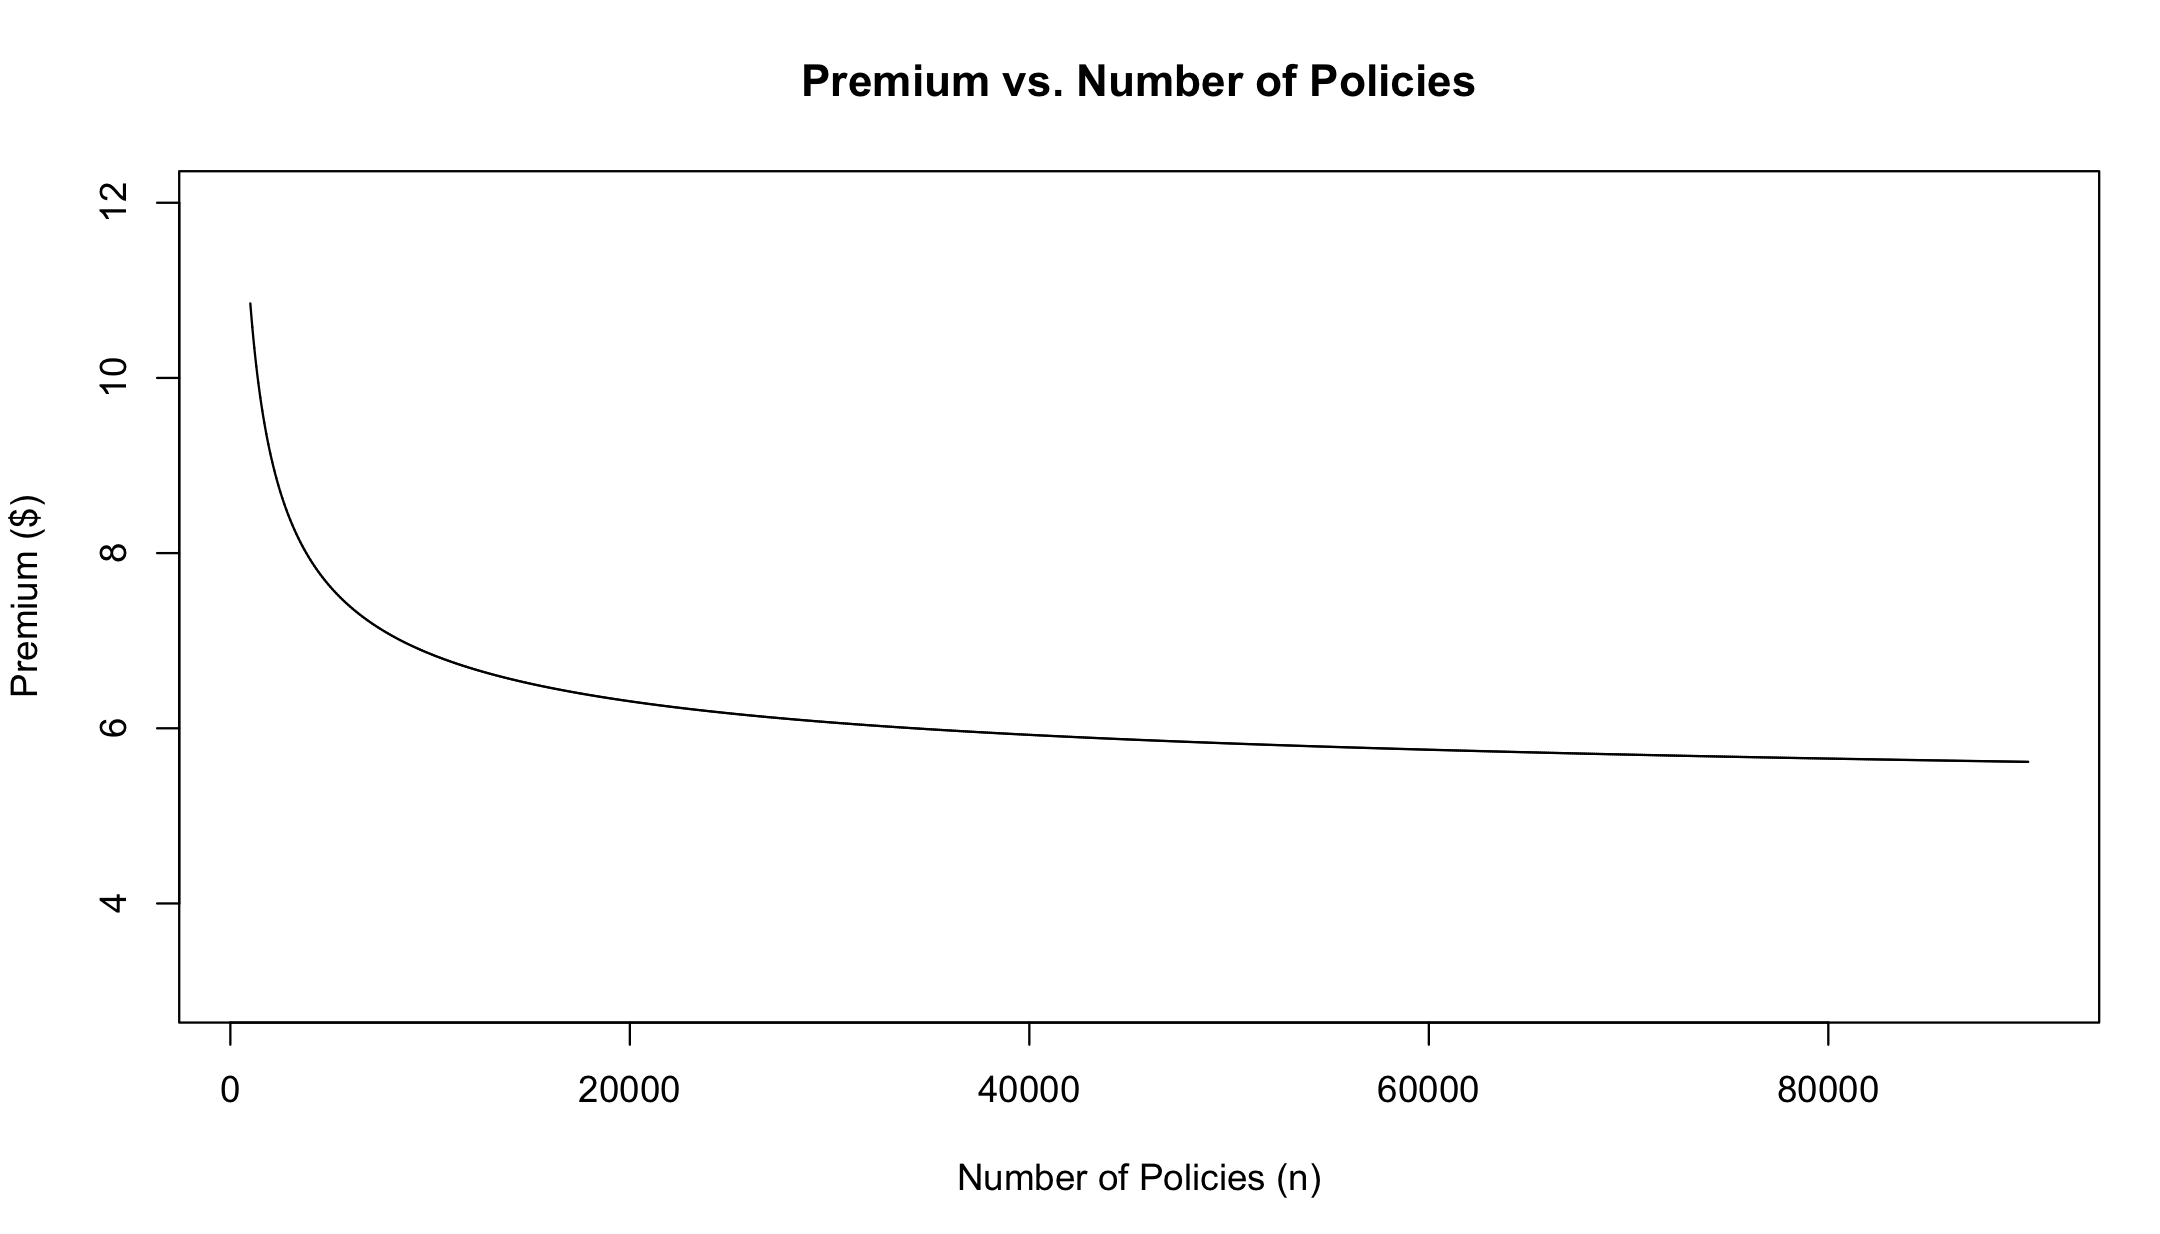
\includegraphics[scale=.35]{premium}
    \end{center}
    \caption{\footnotesize Given $p=0.01$ and $P^*=500$, the premium decreases with the number of policies and slowly approaches $pP^*=\$5$.}\label{fig1}
\end{figure}

\subsection{Premiums as an independent variable}

For the majority of this paper, we assume that $P^*$ is a parameter, and that the premium $P(n)$ is calculated as an output. However, we need not necessarily specify an insurance scheme's payout $P^*$, but instead calculate it from a fixed $P$ by simply solving for $P^*(n)$ in (\ref{premiumpi}). Note that whether starting with $P$ or $P^*$ as the independent variable, the return of this insurance scheme remains constant. In particular, from (\ref{return}) and (\ref{premiumpi}), we see that
$$r = \frac{P^*}{P} = \frac{n}{k(n)}$$
\noindent Indeed, it can be shown that $r(n) \to 1/p$ as $n\to\infty$ and that $r(n) \leq 1/p$ for all $n$. This relationship implies an upper bound of the return for any insurance scheme. This means that a scheme on rare events with, say, $p=0.01$ cannot pay out more than a $100$-fold return, while really common events with, say, $p=0.5$ cannot be insured for more than $2$ times the premium.

\subsection{Calculating expected revenues}

Revenue is an important aspect of our model, since any insurance scheme will need revenue to incentivize stakeholders as well as provide economic interest payments to reinsurers. In this section, we will describe the \textit{revenue}, \textit{revenue margins}, and \textit{reinsurance returns} of the scheme. 

\subsubsection{Revenue}

The \textit{revenue} of our insurance pool is the excess capital that remains in our insurance pool after all of the due claims have been paid; in other words, we define the revenue as
\begin{equation}
    \label{revenue}
    R = C-XP^* = \left(k-X\right)P^*.
\end{equation}
Note that the expected revenue is $E(R)=(k-np)P^*\geq 0$ and, moreover, that $E(R)\to\infty$ as $n\to\infty$. In other words, if the model behaves, it captures an expectation of revenue. The standard deviation of revenue is a straightforward calculation and is, intuitively, proportional to the standard deviation of $X$: $$\sigma_R = P^*\sqrt{np(1-p)} = (P^*)\sigma_X.$$ 

\subsubsection{Revenue margins}

Another useful metric for measuring revenue is the percentage portion of the premium income conserved after claims have been paid. Let us define the \textit{revenue margin} as
\begin{equation*}
    M := \frac{R}{C} = 1 - X\frac{P^*}{nP(n)} = 1-\frac{1}{k}X.
\end{equation*}
With a straightforward calculation, the expectation and standard deviation of $M$ are given by
\begin{equation}
  \label{revmargin}
  E(M) = 1-\frac{np}{k(n)}\ ;\ \ \sigma_M = \frac{1}{k(n)}\sqrt{np(1-p)} = \frac{1}{k}\sigma_X
\end{equation}
Since also $E(M) = 1-pr(n)$ and, since $r(n)$ is positive and bounded above by $1/p$, that $0\leq E(M)\leq 1$. Also, note that $E(M)\to 1$ as $n\to\infty$, as expected. Suppose we want to find the probability that our revenue margin is higher than some level $l$ ($0\leq l\leq 1$). Then from the definition, we have
\begin{equation}
    P(M > l) = P\left(X <(1-l)k\right) = B_{n,p}((1-l)k) \approx \Phi_{\mu,\sigma^2}\left((1-l)k\right)
\end{equation}
where $\Phi_{\mu,\sigma^2}$ is a normally distributed cumulative distribution function with the mean and variance of $X$.

\begin{figure}[H]
    \begin{center}
        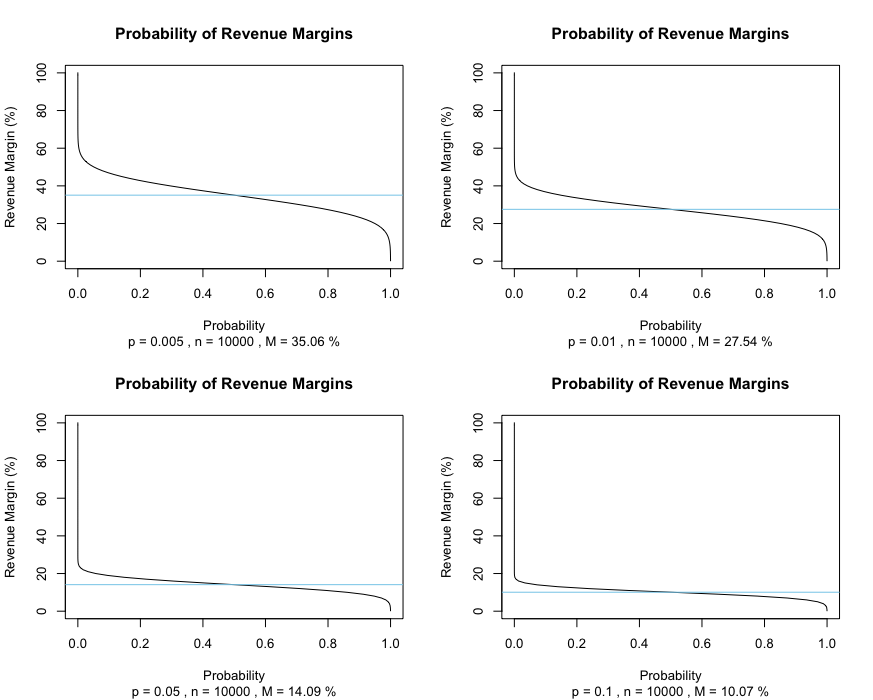
\includegraphics[scale=.5]{margins}
    \end{center}
    \caption{\footnotesize Probability distributions of revenue margins given different values of event probability $p$.}\label{fig1}
\end{figure}

\subsubsection{Reinsurance returns}

Note that after taking on $C(n)$ worth of collateral, our scheme has $L(n)-C(n) =(n-k)P^*$ of potential liability left, and we might be able to transfer this long-tail liability to a reinsurance market. To get a sense of the rate of return for purchasers of the reinsurance, we define the \textit{reinsurance return} as the return over the amount of reinsurance liability on offer.
\begin{equation}
  \tilde{R} := \frac{R}{(n-k)P^*} = \frac{k-X}{n-k}.
\end{equation}
Through a straightforward calculation we get:
$$E(\tilde{R}) = \frac{k - np}{n-k}\ ;\ \ \sigma_{\tilde{R}} = \frac{\sqrt{np(1-p)}}{n-k} = \frac{1}{n-k}\sigma_X.$$

\subsection{Summary}

In summary, a Bernoulli distribution insurance scheme allows us to calculate a premium $P(n)$ from a fixed parameter payout $P^*$ for insuring against events which occur with probability $p$ and to maintain solvency in the scheme with probability $\pi$. Other properties of this scheme include:

\begin{enumerate}
    \item Insurance premiums grow as the probability $p$ of the insurable event grows.
    \item The return of the insurance scheme improves as the number of policies $n$ grows, but it is bounded above by $1/p$.
    \item As the number of policies $n$ grows the premium falls, but it is bounded below by $pP^*$.
    \item We can arbitrarily improve the probability of solvency of the scheme by fixing a sufficiently high $\pi$.
    \item We can specify either a premium or a payout as a parameter.
    \item The revenue margin is the percent of the capital pool that remains after all claims have been paid. The revenue margin is expected to be non-negative with probability $\pi$, and is expected to decrease as the number of policies increases. Revenue margins also decrease as $p$ grows.
\end{enumerate}

\subsection{Concrete example of calculations}

In this section, we outline the steps required to calculate the outputs of our model given the inputs.

\begin{enumerate}
  \item Define the parameters $p$, $n$, $P^*$, and $\pi$. Set $n=10,000$, $p=0.01$, $P^*=\$500$, and $\pi=.9999$.
  \item Note that the number of expected claims is $\mu = np = 10000\cdot .01 = 100$.
  \item Note that the standard deviation of claims is $\sigma = \sqrt{np(1-p)} \approx 9.9499$.
  \item Find $k(n) \approx \Phi^{-1}_{\mu,\sigma^2}(\pi)$, the number of claims that need to be collateralized, by using the normal quartile function; $k(n) \approx \lceil137.0037468\rceil = 138$.
  \item Calculate the premium $P=138/10000\cdot 500 = \$6.90$.
  \item Note that the total collateral will be $C(n) = nP = \$69,000$ and that $r = 500/6.90 \approx 72.46$. The total liability $L(n) = nP^* = \$5,000,000$, so this amount of capital represents a 1.38\% collateralization.
  \item The expected revenue is $E(R) =10000\cdot(6.90-.01\cdot 500)= \$19,000$ and the standard deviation of revenue is $\sigma_R = 500 \cdot 9.9499 = \$4,974.94$. The expected revenue margin is $E(M) = 27.54\%$ and the standard deviation of the revenue margin is $\sigma_M = 7.21\%$.
\end{enumerate}

\section{Extended model with variable payouts}

\subsection{Variable payouts and probabilities}

So far, we have assumed a constant parameter $p$ for each event $X_i$ ($i=1,\ldots,n$). However, we may wish to extend our model to variable payouts and premiums, as well as have the probabilities of insurable events vary across events.

Let $X_i$ be independent Bernoulli variables with $P(X_i = 1) = 1 - P(X_i = 0) = p_i$ for $i=1,\ldots,n$. With each event $X_i$ associate a payout $P^*_i$ and a corresponding premium $P_i$. Then the total outflow of capital to pay for claims is described by
\begin{equation}
  X = \sum_{i=1}^n P_i^* X_i.
\end{equation} 
In this scenario, our capitalization and liability are given by
\begin{equation*}
    C(n) := \sum_{i=1}^nP_i\ ;\ \ L(n) := \sum_{i=1}^n P_i^* 
\end{equation*}
If $F_X$ is the cumulative distribution function of $X$ and $\pi$ is the probability of portfolio solvency, then quantile function $F_X^{-1}$ represents the $\pi$-percentile liability. Our model is then described by
\begin{equation}
  \label{insurance2}
    C(n) = F_X^{-1}(\pi).
\end{equation}
There are many ways to define $P_i$, but the most straightforward is to assume that each premium value $P_i$ is proportional to the associated payout $P_i^*$. In this case, we can define $$P_i := \frac{P_i^*}{\sum_j P_j^*} F_X^{-1}(\pi)$$ and it is clear that (\ref{insurance2}) holds. The mean and standard deviation of the variable payouts model are given by $$E(X) = \sum_{i=1}^np_iP_i^*\ ;\ \ \sigma_X = \sqrt{\sum_{i=1}^np_i(1-p_i)(P_i^*)^2}.$$


\iffalse
\section{Reinsurance model}

We have so far presented a model for insurance which works and produces revenue $\pi$ percent of the time. However, we now turn to the long-tail risk and present one approach of re-selling long-tail risk to a reinsurance market. Consider that the insurance pool has $n-k(n)$ uncollateralized policies and $\mathcal O = L(n)-C(n)=(n-k(n))P^*$ of uncollateralized liability; additionally, the pool has an expected revenue of $R$.

This suggests a basic framework for reselling the long-tail risk through digital tokenization, namely, to tokenize the uncollateralized liability into $m$ tokens where $m := \lceil(n-k(n))P^*\rceil$ and to entitle each token to a return of $R/m$. Whereas $\mathcal O$ is the total liability on offer to the reinsurance market, let us denote as $\mathcal O_0$ the actual reinsurance capitalization the reinsurance pool manages to collect.

We note that because the reinsurance market in a cryptomarket context is an unknown, we can end up with three scenarios:

\begin{enumerate}
  \item $\mathcal O_0$ will be so small that long-tail policies will experience negative returns.
  \item $\mathcal O_0$ will enable all long-tail policies to break even.
  \item $\mathcal O_0$ will be large enough that long-tail policies will experience positive returns.
  \item $\mathcal O_0$ will equal (or exceed) the total liability $\mathcal O$ on offer, and the long-tail risk will be completely offset.
\end{enumerate}
\fi

\end{document}
